\documentclass[pdftex,english,oribibl]{llncs}

%% Spracheinstellungen laden
\usepackage[english]{babel}

%% Schriftart in der Ausgabe/Eingabe
\usepackage[T1]{fontenc}
\usepackage{textcomp}
\usepackage[latin1]{inputenc}

%% Zitate
\usepackage[numbers]{natbib}
\bibliographystyle{abbrvnat}
%\bibliographystyle{dinat}
%\bibliographystyle{plainnat}
%\bibliographystyle{splncs}
%% Similar to option "sectionbib" but \refname instead of \bibname
\makeatletter
\renewcommand\bibsection{\section*{\refname\@mkboth{\MakeUppercase{\refname}}{\MakeUppercase{\refname}}}}
\makeatother

%% Index
%\usepackage{makeidx}
%\makeindex

%% PDF Einstellungen
% muss nach natbib geladen werden!
\usepackage{nameref}
\usepackage{varioref}
\usepackage[pdfusetitle,pdftex,colorlinks]{hyperref}
\hypersetup{pdfborder={0 0 0}}
\hypersetup{bookmarksdepth=3}
\hypersetup{bookmarksopen=true}
\hypersetup{bookmarksopenlevel=1}
\hypersetup{bookmarksnumbered=true}
\usepackage{color}
\hypersetup{colorlinks=false}
\usepackage{titling}
\usepackage{float}

%\usepackage[section]{tocbibind}

\makeatletter
\gdef\@keywords{}
\def\keywords#1{\gdef\@keywords{#1}}
\gdef\@subtitle{}
\def\subtitle#1{\gdef\@subtitle{#1}}

%% modified from llncs
\renewenvironment{abstract}{%
  \list{}{\advance\topsep by0.35cm\relax\small%
          \leftmargin=1cm%
          \labelwidth=\z@%
          \listparindent=\z@%
          \itemindent\listparindent%
          \rightmargin\leftmargin}%
          \item[\hskip\labelsep\bfseries\abstractname]}{%
  \if!\@keywords!\else{\item[~]\item[\hskip\labelsep\bfseries\keywordname]\@keywords}\fi%
  \endlist}

\AtBeginDocument{%
  \if!\@subtitle!\else\hypersetup{pdfsubject={\@subtitle}}\fi
  \if!\@keywords!\else\hypersetup{pdfkeywords={\@keywords}}\fi
}
\makeatother

% llncs hyperref fix
\makeatletter
\providecommand*{\toclevel@author}{0}
\providecommand*{\toclevel@title}{0}
\makeatother

%% Grafiken
\usepackage[pdftex]{graphicx}
\DeclareGraphicsExtensions{.pdf,.jpg,.png}
\usepackage{subfigure}
\usepackage{tikz}
\usepackage{pgfplots}
\usetikzlibrary{shapes,arrows,positioning}
\usepackage{pgfplotstable}
\pgfplotsset{compat=newest}

%% Mathe
\usepackage{amsmath}
\usepackage{amssymb}

%% Listings
\usepackage{listings}
\lstset{escapechar=\%, frame=tb, basicstyle=\footnotesize}

%% Sonstiges
\newcommand{\TODO}[1]{\par\textcolor{red}{#1}\marginpar{\textcolor{red}{TODO}}}
\newcommand{\TODOX}[1]{\textcolor{red}{#1}\marginpar{\textcolor{red}{TODO}}}
\pagestyle{plain}

% Keine "Schusterjungen"
\clubpenalty = 10000
% Keine "Hurenkinder"
\widowpenalty = 10000 \displaywidowpenalty = 10000

%%%%%%%%%%%%%%%%%%%%%%%%%%%%%%%%%%%%%%%%%%%%%%%%%%%%%%%%%%%%%%%%%%%%%%%%%%%%%%%
%%% BEGIN DOCUMENT
%%%%%%%%%%%%%%%%%%%%%%%%%%%%%%%%%%%%%%%%%%%%%%%%%%%%%%%%%%%%%%%%%%%%%%%%%%%%%%%
\pretitle{%
  \begin{center}\LARGE
  \noindent
\includegraphics[height=2.5cm]{figures/logo-se}\hfill{}
\includegraphics[height=2.5cm]{figures/logo-uni}\\\vspace{0.5cm}
}
\title{Whole Test Suite Generation with \textsc{EvoSuite}}
% \subtitle{My (optional) Subtitle}
\author{Nguyen, Hoang Lam \\ Peverali, Francois \\ Allogie, Mohamad Jamal}
\institute{Humboldt University of Berlin\\Department of Computer Science\\12489 Berlin, Germany}
\posttitle{\end{center}}


\begin{document}

\maketitle

\begin{abstract}
In the context of search based software testing, existing studies have shown that for object-oriented software systems, the whole test suite approach leads to higher coverage than the traditional single-goal approach \cite{Fraser2011,Fraser2013,Rojas2017}. Recently, Scalabrino et al. \cite{Scalabrino2016} have investigated whole test suite approaches for procedural programs and have introduced an iterative single-goal search strategy, which they refer to as Linearly Independent Path based search (LIPS). In the conducted experiments, the proposed LIPS approach provided a higher efficiency while achieving the same or even higher coverage than the whole test suite approach, opposing the results of existing studies conducted on object-oriented software systems. 

We have implemented the proposed LIPS approach in \textsc{EvoSuite}. The approach has been evaluated on 10 classes of the Joda-Time library against the traditional single-goal approach as well as the whole test suite approach. Contrary to the results of Scalabrino et al., the proposed approach did not outperform the whole test suite approach in our experiments.
\end{abstract}

\section{Introduction}

Software products are inherently error prone and therefore software developers need efficient methods and techniques to test their programs against possible faults. Testing of software is a lengthy procedure and therefore related to high costs because it does not add any value to the final product. Still, it is a necessary activity, since a high code coverage by test cases reduces bugs and thereby faulty program behavior. Therefore helping developers with the activity of software verification by automatically generating test cases is a welcome approach to this issue.
Given a source code of a program, there are different approaches to automated test case generation to help the developer find bugs in the software. There are  many tools which automatically generate test cases, that implement different approaches. They all share three fundamental parameters, which are given by the coverage, the redundancy (of test cases or statements within test-cases) and spent time for the test case generation, that are related to each other. We can differentiate between three basic approaches for automated white-box testing: the varying aims of test-case generation techniques consist either in approximating the test coverage of a specified line (though a fitness function), optimizing a single goal, which could be a determined class, by converging towards a coverage criterion for this specific program context or -- last, not least -- in whole test suite optimization through a coverage criterion. 
The latter is adopted by \textsc{EvoSuite} which is discussed by Fraser and Arcuru \citet{Fraser2011}.
As an whole test suite generation tool \textsc{EvoSuite} generates both tests and assertions for Java Classes. More exactly it restricts the oracle problem with a mutation based approach, which is a key problem in automated software testing and basically consists in minimizing possible assertions for a given set of tests. 

%Hier sollte das problem single-goal vs. whole test suite optimization motiviert werden (vor/nachteile). Diese Ansaetze werden dann im Background naeher erlaeutert bzw. spezifiert.

%This is a crucial issue since automated test generation often overfulfils its aims by creating tests which are in one and the same equivalence class thereby confronting the testing developer with a high number of inefficient test-cases and the difficulty to choose and discard the ones that are not needed or redundant for testing a certain program behavior. Moreover, \textsc{EvoSuite} offers the choice between several coverage criteria for the test suite's optimization, i.e. line, branch output and mutation testing. In so doing it also provides different metrics to analyze a given test suite, which is another feature it provides. \textsc{EvoSuite} is provided as a command line tool but offers as well Integration for multiple IDEs and platforms like Eclipse, IntelliJ and Maven.
%This paper aims at validating the \textsc{EvoSuite} approach by providing further empirical data on the effectiveness of test suite optimization in comparison to both a traditional approach and the so called LIPS method for automated test case generation.


\section{Background}

Software-testing within software-engineering deals with systematically verifying the functionality of the tested program and thereby assuring its quality. In order to increase the efficiency of writing test-cases, automated methods that seek to generate test-cases by iterating through a possible search-space are being used. A comprehensive comparison of both a traditional and a novel approach in search-based software testing is offered by Rojas et al. \citep{rojas2017detailed}. A common scenario for software-based software testing consists in generating "a set of test cases maximizing their code coverage or maximizing their fault detection capability" being branch coverage a de facto standard coverage criterion within the reasearch field. Furthermore it states that the traditional approach can be characterized as a single goal approach, i.e. that each coverage goal is approximated individually. Whereas for the novel \textit{whole test suite} approach proposed by Rojas et al. "the problem is changed to a search for a set of tests that covers all coverage goals at the same time", thereby solving two issues of the traditional approach, which are given by the \textit{search budget distribution problem} and the \textit{ordering of the coverage goals}. The former consisting in the fact, that the infeasibility of coverage goals is an undecidable problem, which means that a test generation software could unnecessarily spend ressources on test generation for a coverage goal that could never be reached. The latter consisting in the fact that each goal is tipycally approximated individually and useful information is not shared between the single search processes. 

A detailed description for the traditional approach is provided by McMinn \citep{mcminn2004search} and Wegener \citep{wegener2001evolutionary},  whereas a more detailed description of the whole test suite approach can be found at Fraser and Arcuri \citep{fraser2015achieving}.


\subsection{Linearly Independent Path based Search (LIPS)}
Recently, Scalabrino et al. \cite{Scalabrino2016} have investigated whole test suite approaches in the context of procedural programs. For their study, they have implemented a tool called \textsc{OCELOT} (Optimal Coverage sEarch-based tooL for sOftware Testing), which is able to generate test suites using state-of-the-art whole test suite approaches as well as a novel iterative single-target approach, which they refer to as Linear Independent Path based Search (LIPS). The proposed LIPS approach aims to target the key issues of single-goal approaches: choosing a coverage goal order and efficiently distributing the search budget.

Inspired by Dynamic Symbolic Execution, the search algorithm starts with a randomly generated test case $t_0$. The not covered branches along the execution path of $t_0$ are then added to a worklist. Afterwards, the last branch added to the worklist is removed and used as the next target of the search algorithm. If the genetic algorithm is able to cover this goal, a new test case $t_i$ is added to the test suite and the branches not covered along the execution path of $t_i$ are added to the worklist (unless they are already in the worklist). This procedure is repeated until the worklist is empty (i.e. all branches are covered) or until the search budget is entirely consumed. Note that by choosing the last added branch to the worklist as the next goal and reusing the final population of the previous iteration as the next population, the genetic algorithm is expected to more efficiently generate a test case that covers the selected branch.

In order to avoid wasting search budget on infeasible goals, LIPS uses a dynamic allocation of the search budget. Specifically, at each iteration of the test generation process, the remaining budget is equally distributed over the remaining goals.


%\vspace{-5cm}
\begin{figure}[t]
%\vspace{0.5cm}
%\hspace{1cm}
\begin{minipage}[ht]{.4\textwidth}
\centering
\begin{lstlisting}[language=Java,basicstyle=\ttfamily,keywordstyle=\bf,numbers=left,frame=tlrb,tabsize=5,firstnumber=1]{Name}
int foo(int x){
  if(x != 10){
    if(x > 15){
      x = 15;
    }
    else{
      x = 0;
    }
  }
  if(x > 20){
    x = 20;
  }
  return x;
}
\end{lstlisting}
\label{fig:lips_code}
\end{minipage}
%\hspace{1cm}
\begin{minipage}[ht]{.4\textwidth}
\centering
%\vspace{5cm}
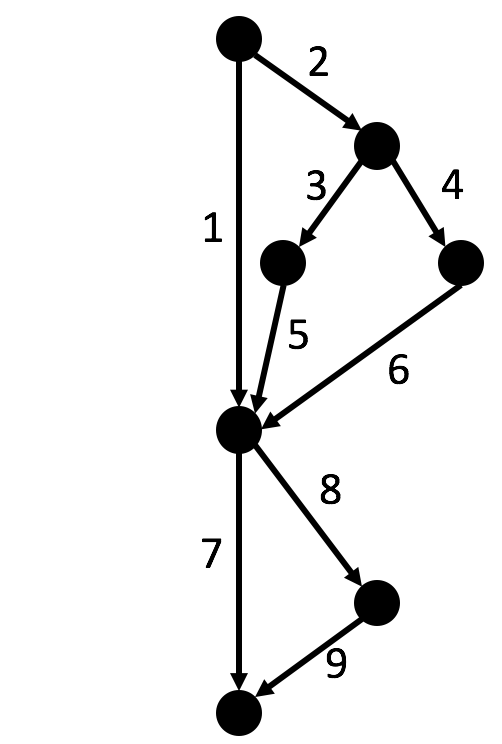
\includegraphics[scale=0.5]{figures/cfg.png}
\label{fig:lips_cfg}
\end{minipage}
\caption{Example program and its control flow graph to illustrate the LIPS search strategy. At every decision node, the right and left child node denote the true and false branch, respectively.}
\label{fig:lip}
\end{figure}

As an illustration, consider the example code and respective control flow graph in Figure \ref{fig:lip}. Assume further that the initial test case \texttt{foo(10)} has been randomly generated, which covers the branches 1 and 7. The branches which have not been covered along the execution path are branch 2 and 8 
and are therefore added to the worklist. Since branch 8 has been added last, it is chosen as the next goal. A test case which covers this goal could be for example \texttt{foo(21)}, which also covers the branches 2, 4, 6 and 9 due to collateral coverage. The only branch along the execution path of this test case, which has not been covered yet, is branch 3. Generating a test case for this branch leads to full branch coverage, since branch 5 will also be covered.

\newpage
\section{Evaluation}
We have implemented the LIPS approach as an additional search strategy for \textsc{EvoSuite}. The goal of the experiments was to compare the LIPS approach to the whole test suite generation approach as well as the traditional single-goal approach. When comparing the different algorithms, we measured the branch coverage of the generated test suites, which is computed as the fraction of program branches executed by the test suite. 
\subsection{Case study subjects}
For our evaluation, we chose the Joda-Time\footnote[1]{\url{https://github.com/JodaOrg/joda-time}} library, which is an open-source library for working with dates and times, including various date-time calculations. It was originally developed as an alternative for the Java date and time classes, but has been replaced by the \texttt{java.time} API included in Java SE 8. We have evaluated the different approaches on 10 classes of the Joda-Time library. An overview of the case study subjects is given in Figure \ref{fig:subjects}.

\begin{figure}[h] 
\centering
\begin{tabular}{l c c} \hline
Class & \#Branches & LOC\footnote[1]{} \\ \hline
DateMidnight & 117 & 96 \\
DateTime & 168 & 620 \\
DateTimeComparator & 54 & 101 \\
DateTimeField & 1 & 54 \\
DateTimeFieldType & 133 & 299 \\
DateTimeUtils & 57 & 206 \\
DateTimeZone & 194 & 577 \\
Days & 65 & 160 \\
Hours & 67 & 163 \\
LocalDate & 221 & 654 \\ \hline
$\Sigma$&1077&2930 
\end{tabular}
\caption{Number of branches and LOC of the case study subjects. LOC (Lines of code) is the number of non-comment source code lines and was computed using cloc (\url{https://github.com/AlDanial/cloc}).\label{fig:subjects}}
\end{figure}

\subsection{Experimental Setup}
The experiments were essentially run on the standard configuration of \textsc{EvoSuite}. \textsc{EvoSuite} itself is highly configurable, for example it is possible to set several parameters (e.g. crossover and mutation probability) and to choose between different genetic algorithms and search strategies. However, we decided against modifying any parameters (except for the timeout, which has been set to 90 seconds) because the tool already comes with tuned parameters. 

Since the search strategy of \textsc{EvoSuite} is based on randomized algorithms, different runs may produce different results. For this reason, we have run each experiment three times in a row and computed the average branch coverage.

The experiments were conducted on a machine running macOS 10.12.5 featuring an 2,6 GHz Intel Core i5 and 16 GB of memory.




\begin{figure}[h]
%0 - aramente   1 - �s vezes   2 - Quase sempre   4 - Sempre
\pgfplotstableread{
  %2013-2014    %2012-2013  %2011-2012
0 0.97 0.33 0.44
1 0.96 0.22 0.32
2 0.93 0.41 0.7
3 1.0 1.0 0.0
4 0.57 0.24 0.0
5 0.92 0.63 0.22
6 0.81 0.3 0.23
7 0.98 0.6 0.89
8 0.99 0.53 0.85
9 0.94 0.31 0.38
}\dataset
\hspace{-3.7cm}
\begin{tikzpicture}
\begin{axis}[ybar,
        width=20cm,
        height=8cm,
        ymin=0,
        ymax=1,
        ylabel={Branch Coverage},
        xtick=data,
        xticklabels = {
            \strut Class 1,
            \strut Class 2,
            \strut Class 3,
            \strut Class 4,
            \strut Class 5,
            \strut Class 6,
            \strut Class 7,
            \strut Class 8,
            \strut Class 9,
            \strut Class 10
            %Category 5,
            %Category 6
        },
        %xticklabel style={yshift=-10ex},
      enlarge y limits={abs=0.15,upper},
        major x tick style = {opacity=0},
        minor x tick num = 1,
        minor tick length=2ex,
        every node near coord/.append style={
                anchor=west,
                rotate=90
        },
        	%legend style={at={(1,-0.1)},
        legend entries={EvoSuite ,Traditional ,LIPS },
        legend columns=3,
        legend style={draw=none,nodes={inner sep=3pt},at={(0.625,-0.1)}},
        ]
\addplot[draw=black,fill=blue!20, nodes near coords] table[x index=0,y index=1] \dataset; %ano de 2013-2014
\addplot[draw=black,fill=blue!40, nodes near coords] table[x index=0,y index=2] \dataset; %ano de 2012-2013
\addplot[draw=black,fill=blue!60, nodes near coords] table[x index=0,y index=3] \dataset; %ano de 2011-2012
\end{axis}
\end{tikzpicture}

\centering
\vspace{0.3cm}
\begin{tabular}{l c c } \hline
Approach & Avg. coverage & Avg. Length\\ \hline
EvoSuite & 0.88 & 130.8\\ 
Traditional & 0.33 & 37.6\\
LIPS & 0.38& 59.5 \\\hline
\end{tabular}
\caption{Branch coverage achieved by each approach\label{fig:diagram}}
\end{figure}

\newpage
\subsection{Results}
Figure \ref{fig:diagram} gives a detailed overview of the coverage achieved by each approach. Overall, the whole test suite approach clearly outperforms the traditional single-goal and LIPS approach with an average branch coverage of $0.88$. While the LIPS approach seems to generate higher coverage test suites (despite being unable to cover any branch in two instances), the difference to the traditional single-goal approach is likely not significant. When reviewing the individual runs of the LIPS approach, the number of covered branches varied greatly, which indicates that the LIPS approach heavily relies on the initial test case. On the other hand, the traditional single-goal approach performed more stable results.

\section{Conclusions and Future Work}\label{sec:conclusions}
Recently, Scalabrino et al. \cite{Scalabrino2016} have investigated whole test suite approaches for procedural programs and have introduced an iterative single-goal search strategy (LIPS) that aims to mitigate the key issues of the single-goal approach. 
We have implemented the proposed LIPS approach as an extension to the traditional single-goal strategy in \textsc{EvoSuite} (which standardly uses a whole test suite approach). Contrary to the results of Scalabrino et al., the approach was unable to outperform the whole test suite approach and even performed worse than the traditional single-goal approach in some instances. Further inspection of the results indicate that the performance of the LIPS approach heavily relies on the initial test case.

Future work could include running the experiments on a larger scale in order to get more generalizing results. If the LIPS approach still does not perform as expected, the underlying reasons for this result should be further investigated. On the other hand, one could also try to further optimize the approach, e.g. by heuristically choosing the initial test case, since it seems to have a big impact on the performance. Moreover, analyzing how well the LIPS approach performs over time could possible open up new possibilities for hybrid-approaches. 

\section{Related Work}
The closest to our work is the work by Fraser and Arcuri \cite{Fraser2011,Fraser2013}, who have conducted empirical studies on the whole test suite approach with \textsc{EvoSuite} and showed that it can achieve a higher code coverage than the traditional single-goal approach. Since these studies have been carried out on object-oriented software systems, Scalabrino et al. \cite{Scalabrino2016} have studied whole test suite approaches in the context of procedural programs where they also introduced a novel single-goal approach. The approach, which they refer to as Linearly Independent Path based search (LIPS), performed better than the whole test suite approach in the experiments. In our studies, we tried to reproduce the results in the context of object-oriented programs using \textsc{EvoSuite}.

%Furthermore Rojas et al. \citep{rojas2017detailed} have analyzed in-depth possible problem sources of the novel approach caused by the fact that a higher code coverage does not necessarily imply that all cases of the traditional approach are covered by the whole test suite approach. They've come to the conclusion that there are in fact specific contexts in which a single goal approach can outperform the whole test suite approach even on code coverage, still being "special cases, rather than general efficiencies of the approach", which -- as they show -- can be improved by adding an "archive", which still needs further research. Our evaluation of \textsc{EvoSuite} validates the findings of Fraser and Arcuri \cite{fraser2013whole} by using the tool for test suite optimization on another buggy software (...) the results of the code coverage of adopting \textsc{EvoSuite} show to outperform the single goal approach used as comparison... 



\bibliography{bibliography.bib}

\end{document}
